\documentclass[12pt,a4paper]{article}
\usepackage[spanish,es-tabla]{babel}
\usepackage{float}							% Insertar figuras


\usepackage{subcaption}

\usepackage[utf8]{inputenc} % Escribir con acentos, ~n...
\usepackage{eurosym} % s´ımbolo del euro
\newcommand{\horrule}[1]{\rule{\linewidth}{#1}} % Create horizontal rule command with 1 argument of height
\usepackage{listings}             % Incluye el paquete listing
\usepackage{amsfonts}
\usepackage{booktabs}

\usepackage{amsmath}

\usepackage[cache=false]{minted}
\usepackage{graphics,graphicx, float} %para incluir imágenes y colocarlas
\usepackage{hyperref}
\hypersetup{
	colorlinks,
	citecolor=black,
	filecolor=black,
	linkcolor=black,
	urlcolor=black
}
\usepackage{multirow}
\usepackage{array}
\usepackage{diagbox}
\usepackage{listings}

\lstset{language=Java,
	keywordstyle=\color{RoyalBlue},
	basicstyle=\scriptsize\ttfamily,
	commentstyle=\ttfamily\itshape\color{gray},
	stringstyle=\ttfamily,
	showstringspaces=false,
	breaklines=true,
	frameround=ffff,
	frame=single,
	rulecolor=\color{black}}
\title{
\normalfont \normalsize 
\textsc{{\bf Simulación de Sistemas (2019-2020)} \\ Grado en Ingeniería Informática \\ Universidad de Granada} \\ [25pt] % Your university, school and/or department name(s)
\horrule{0.5pt} \\[0.4cm] % Thin top horizontal rule
\huge Práctica 4: Modelos de Simulación Dinámicos Continuos\\% The assignment title
\horrule{2pt} \\[0.5cm] % Thick bottom horizontal rule

\includegraphics{images/logo.png}	
}

\author{Antonio Jesús Heredia Castillo} % Nombre y apellidos

\date{\normalsize\today} % Incluye la fecha actual

%----------------------------------------------------------------------------------------
% DOCUMENTO
%----------------------------------------------------------------------------------------

\begin{document}

\maketitle % Muestra el Título

\newpage
\tableofcontents % para generar el índice de contenidos
\newpage %inserta un salto de página

\section{Descripción del sistema}

Aunque viene explicado en el Guión de la practica vamos a hacer un pequeño repaso a modo de resumen del sistema que vamos a simular. \\ En esta practica vamos a tratar con el modelo de ecosistema de Lotka-Volterra. Este es un modelo dinámico continuo que consta de dos ecuaciones. 
$$
\begin{aligned}
&\frac{d x}{d t}=a_{11} x-a_{12} x y\\
&\frac{d y}{d t}=a_{21} x y-a_{22} y
\end{aligned}
$$
A continuación describiremos todos los parámetros que corresponde al sistema.
\begin{itemize}
	\item \textbf{x} es la población de presas
	\item \textbf{y} es la población de depredadores.
	\item $\pmb{a_{11}}$ es la tasa de natalidad de las presas
	\item $\pmb{a_{12}}$ es como de efectivos son los depredadores a la hora de cazar a las presas. 
	\item $\pmb{a_{21}}$ es cuantas presas necesita un depredador para poder alimentarse
	\item $\pmb{a_{22}}$ es la tasa de mortalidad de los depredadores. 
\end{itemize}

\section{Experimento inicial} 
Para este y los experimentos que vienen, usaremos el mismo $\pmb{tini} = 0$ $\pmb{tfin} = 150$. Los valores para los distintos parámetros los detallo a continuación. 
\begin{itemize}
	\item $\pmb{a_{11}} = 5$ 
	\item $\pmb{a_{12}} = 0.05$  
	\item $\pmb{a_{21}} = 0.0004$
	\item $\pmb{a_{22}} = 0.2$ 
	\item $\pmb{h} = 0.1$ 
\end{itemize}
Para este punto y los dos siguiente utilizaremos solamente el método de integración de Runge-kutta con el intervalo de cálculo \textbf{h}. El experimento consiste en coprobar qué ocurre cuando las condiciones iniciales son $\pmb{x} = a_{22}/a_{21}$ y  $\pmb{y} = a_{11}/a_{12}$. Ademas investigaremos qué ocurre cuando los valores iniciales de x e y se van progresivamente distanciando de los valores anteriores. Calculamos cual es el valor que vamos a tener para $x=\frac{0.2}{0.0004}=500$ e $y=\frac{5}{0.05}=100$. Probamos el sistema y obtenemos que:


\begin{figure}[H]
	\centering
	\begin{subfigure}{.5\textwidth}
		\centering
	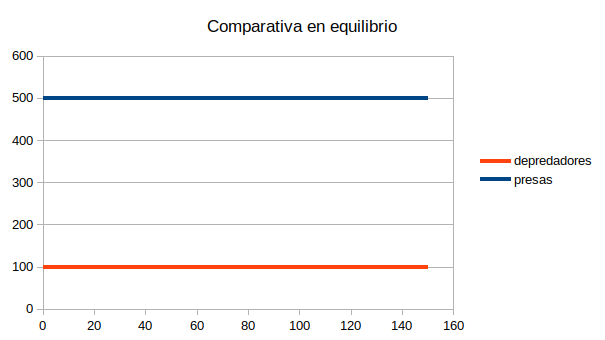
\includegraphics[width=1\linewidth]{images/ejercicio2_1}
		\caption{}
	\label{fig:ejercicio211}
		
	\end{subfigure}%
	\begin{subfigure}{.5\textwidth}
		\centering
	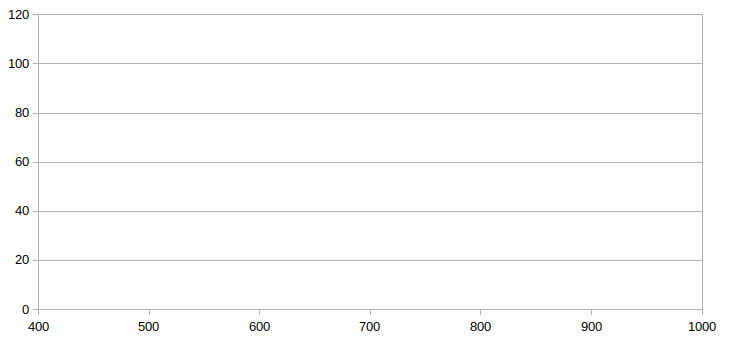
\includegraphics[width=1\linewidth]{images/ejercicio2_1_2}
		\caption{}
	\label{fig:ejercicio212}
	\end{subfigure}
	
	\label{fig:ejercicio21}
\end{figure}
 En la Figura \ref{fig:ejercicio211} podemos ver que la población se mantiene siempre igual. Esto se debe a que como los valores iniciales de \textbf{x} e \textbf{y} son proporcionales a los parametros de configuración del modelo, el crecimiento de uno y la depredación de los otros se mantienen estables en el tiempo. Ahora empezaremos a cambiar en numero inicial de depredadores y presas, para ver como responderá el ecosistema a estos cambios. En la Figura \ref{fig:ejercicio212} no aparece nada ya que todo los puntos en x corresponde a el mismo y. Por lo tanto solo se dibujaria un punto.  		\\Como pone en el guión empezaremos aumentando la distancia entre la cantidad de depredadores y presas.

\begin{figure}[H]
	\centering
	\begin{subfigure}{.5\textwidth}
		\centering
	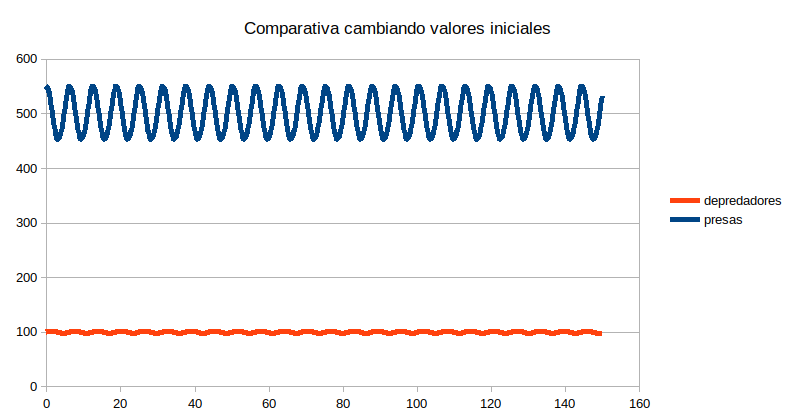
\includegraphics[width=1\linewidth]{images/ejercicio2_2}
		\caption{}
			\label{fig:ejercicio221}

	\end{subfigure}%
	\begin{subfigure}{.5\textwidth}
		\centering
 	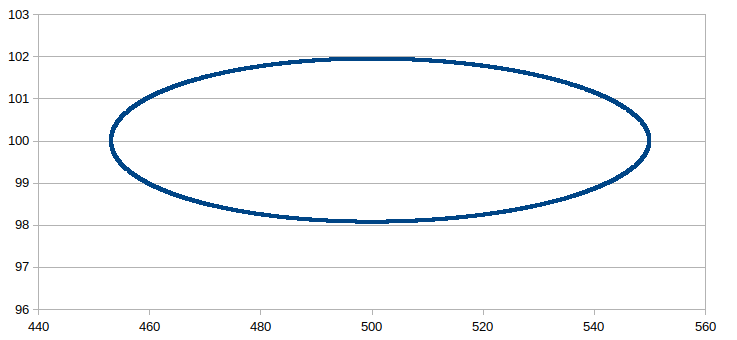
\includegraphics[width=1\linewidth]{images/ejercicio2_3_3}
		\caption{}
 	\label{fig:ejercicio233}
	\end{subfigure}

	\label{fig:ejercicio22}
\end{figure}
En la Figura \ref{fig:ejercicio221} hemos establecido el valor de \textbf{x=550} y hemos mantenido el valor de \textbf{y=100}. Con este pequeño cambio ya podemos observar como la cantidad de animales vivos empieza a fluctuar en ambos. En los momentos que la población de presas aumenta esto permite a los depredadores cazar mas y por lo tanto aumentar su población también. Lo que provoca que vuelvan a decrecer la población de presas. Estas fluctuaciones son las que podemos ver en la Figura \ref{fig:ejercicio221}. De hecho ocurre lo que de manera intuitiva podríamos pensar. Todavía estamos en un modelo en el que el numero de depredadores y presas se pueden mantener estables sin que ninguna de las dos desaparezca. Ademas en la Figura \ref{fig:ejercicio233} podemos ver como pequeños variaciones crean una elipse casi perfecta. Los vértices de la elipse serán los puntos donde los depredadores y presas tienen una población máxima o mínima. 
\\Podemos probar aumentar aun mas la diferencia y ver como actual el sistema. 


\begin{figure}[H]
	\centering
	\begin{subfigure}{.5\textwidth}
		\centering
	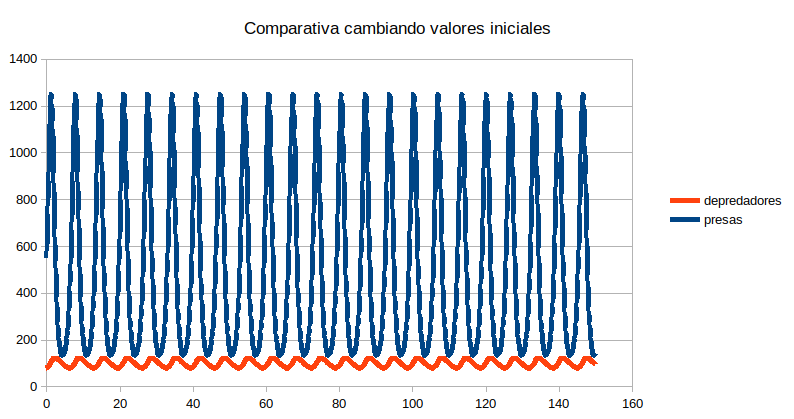
\includegraphics[width=1\linewidth]{images/ejercicio2_3}
		\caption{}
	\label{fig:ejercicio231}
\end{subfigure}%
\begin{subfigure}{.5\textwidth}
		\centering
	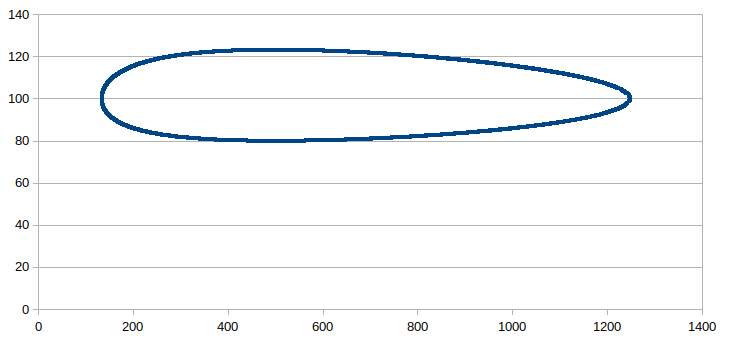
\includegraphics[width=1\linewidth]{images/ejercicio2_3_2}
		\caption{}
	\label{fig:ejercicio232}
	\end{subfigure}

	\label{fig:ejercicio23}
\end{figure}
En la Figura \ref{fig:ejercicio231} ademas de dejar la población de presas a 550 también reducimos en 20 la cantidad de depredadores. Y como podemos ver la fluctuación es aun mas agravada. Podemos ver como parece que afecta mucho mas pequeños cambios en los depredadores que en la población inicial de presas. Para el ultimo experimento que voy a realizar dejare en 500 la población inicial de presas y aumentare a 175 la población inicial de depredadres. 

\begin{figure}[H]
	\centering
	\begin{subfigure}{.5\textwidth}
		\centering
	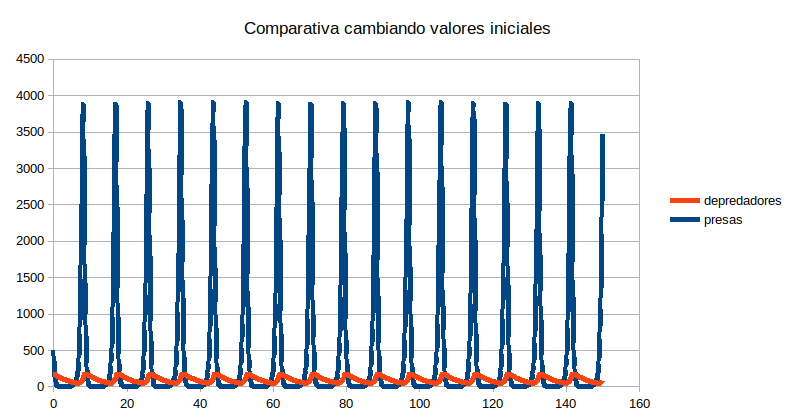
\includegraphics[width=1\linewidth]{images/ejercicio2_4}
		\caption{}
	\label{fig:ejercicio241}
	\end{subfigure}%
	\begin{subfigure}{.5\textwidth}
		\centering
	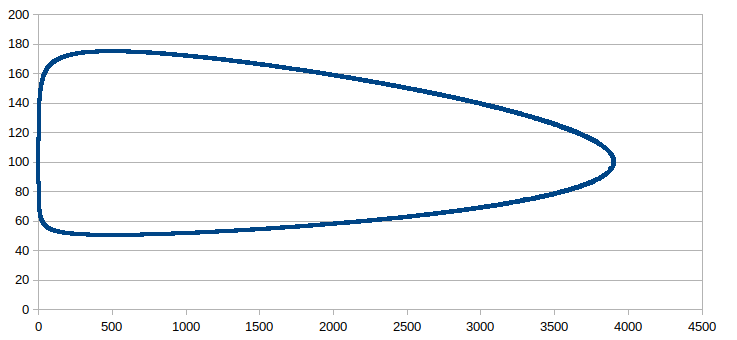
\includegraphics[width=1\linewidth]{images/ejercicio2_4_2}
		\caption{}
	\label{fig:ejercicio242}
	\end{subfigure}

	\label{fig:ejercicio24}
\end{figure}
Como podemos ver en la Figura \ref{fig:ejercicio241} aumentar mucho los depredadores puede provocar que en momentos la población de presas pueda llegar a ser 0 o casi 0. La buena noticia para las presas es que cuando su población es cercana a 0 los depredadores empiezan a descender mucho, permitiendo así que las presas puedan volver a hacer crecer su población de forma muy rápida. 

\section{Probando diferentes $a_{ij}$}
Ahora vamos a realizar experimentos para ver como afecta el cambio a los parámetros $a_{ij}$. Estos parámetros afectan a como de eficaces son los depredadores cazando, a como son las tasas de crecimiento, la longevidad de los depredadores  y cuantas presas necesita un depredador para sobrevivir. \\
Para hacer los experimentos fijaremos $x=500$ e $ y=100$, que sabemos que son estables para los parámetros anteriores pero no sabemos como funcionaran con las modificaciones. 
\subsection{Modificando $a_{11}$}
Ahora vamos a ver como se comporta el sistema si cambiamos la natalidad de las presas. Por ejemplo vamos a hacer que las presas se reproduzcan con mas facilidad. Por ejemplo probaremos como afecta que el factor $a_{11}=7$
\begin{figure}[H]
	\centering
	\begin{subfigure}{.5\textwidth}
		\centering
	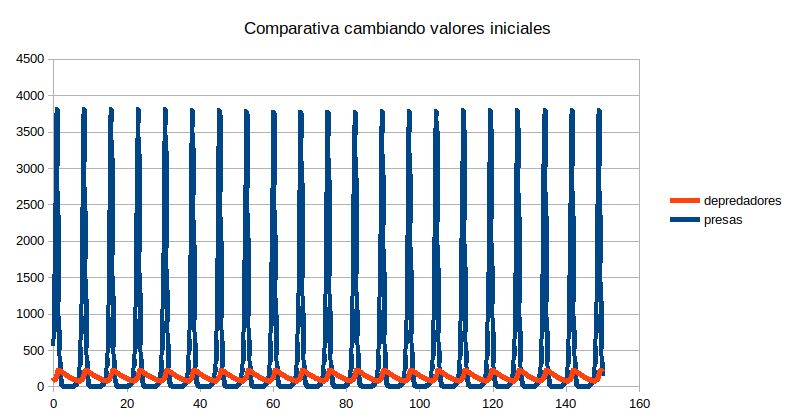
\includegraphics[width=1\linewidth]{images/ejercicio4_1_1}
		\caption{}
	\label{fig:ejercicio411}
	\end{subfigure}%
	\begin{subfigure}{.5\textwidth}
		\centering
	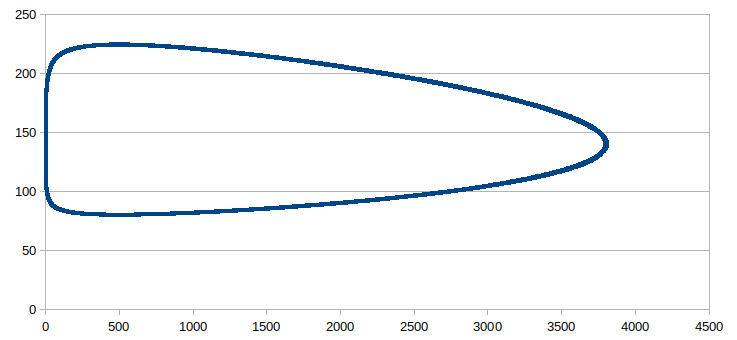
\includegraphics[width=1\linewidth]{images/ejercicio4_1_2}
		\caption{}
	\label{fig:ejercicio412}
	\end{subfigure}
	
	\label{fig:ejercicio41}
\end{figure}

Como podemos ver en la Figura \ref{fig:ejercicio411} al nacer mas presas, la población es fácil que aumente rápidamente. El comportamiento es el mismo que el que esperábamos intuitivamente. Esto es interesante ya que podemos ver como no siempre es recomendable que una especie de animales se reproduzca todo lo que quiera ya que esto puede afectar a que el numero de depredadores suyos también aumente y por lo tanto esta pueda llegar a desaparecer dado el caso. \newpage
\subsection{Modificando $a_{12}$}
En este experimento hemos puesto el valor de $a_{12}=0.1$.  Este valor corresponde con lo eficaz que son los depredadores cazando. Al capturar mas presas la población de las mismas tarda menos en disminuir. 
\begin{figure}[H]
	\centering
	\begin{subfigure}{.5\textwidth}
		\centering
	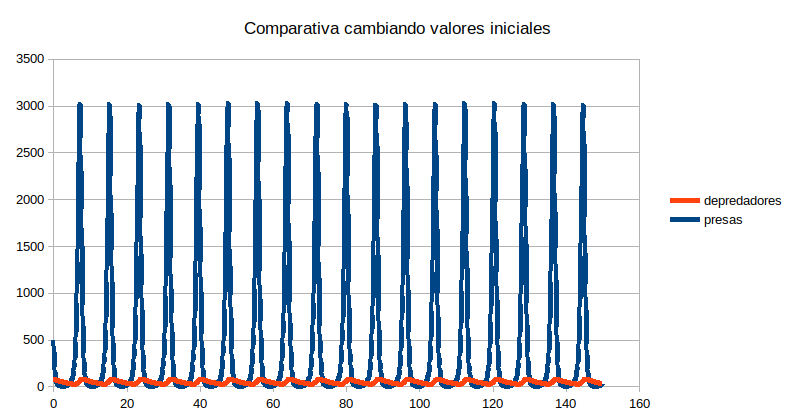
\includegraphics[width=1\linewidth]{images/ejercicio4_2_1}
		\caption{}
	\label{fig:ejercicio421}
	\end{subfigure}%
	\begin{subfigure}{.5\textwidth}
		\centering
	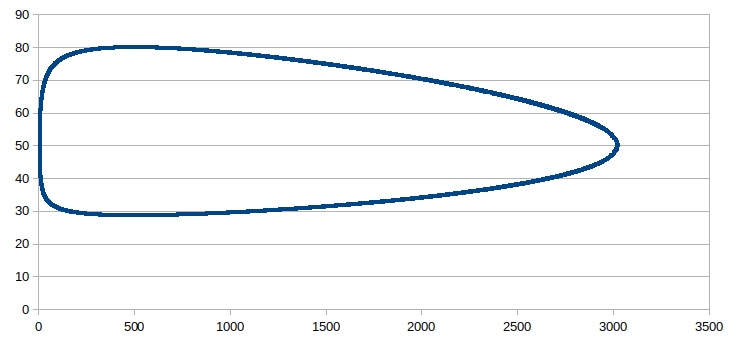
\includegraphics[width=1\linewidth]{images/ejercicio4_2_2}
		\caption{}
	\label{fig:ejercicio422}
	\end{subfigure}
	
	\label{fig:ejercicio42}
\end{figure}
Aunque la Figura \ref{fig:ejercicio421} sea muy parecida a la Figura \ref{fig:ejercicio411}, esto no es asi. La mayor diferencia es que en este caso la población de presas comienza disminuyendo debido a la cantidad de cazas por parte de los depredadores. En el caso del punto anterior la población de presas comenzaba aumentando esto 
\subsection{Modificando $a_{21}$}
En este experimento vamos a probar ver que ocurre cuando modificamos el parametro que nos indica la cantidad de presas que necesita un depredador para vivir. Para ello modificamos $a_{21}=0.02$. 
\begin{figure}[H]
	\centering
	\begin{subfigure}{.5\textwidth}
		\centering
	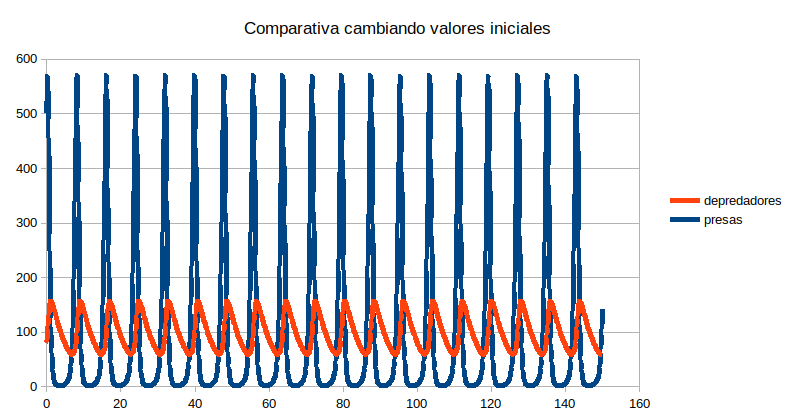
\includegraphics[width=1\linewidth]{images/ejercicio4_3_1}
		\caption{}
	\label{fig:ejercicio431}
	\end{subfigure}%
	\begin{subfigure}{.5\textwidth}
		\centering
	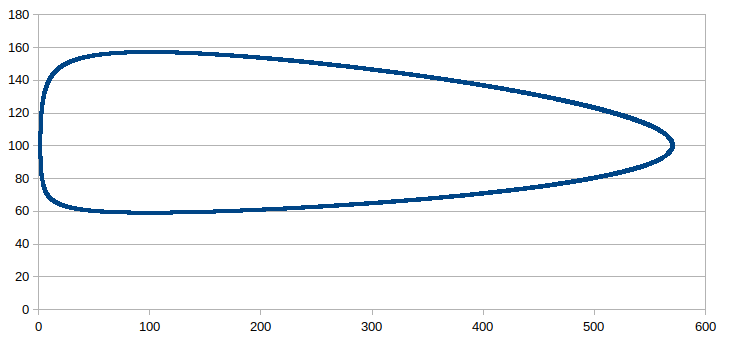
\includegraphics[width=1\linewidth]{images/ejercicio4_3_2}
		\caption{}
	\label{fig:ejercicio432}
	\end{subfigure}
	
	\label{fig:ejercicio423}
\end{figure}
En la Figura \ref{fig:ejercicio431} se puede ver como posiblemente alcancemos los valores para la cantidad de depredadores mas altos. Esto es facilmente comprensible debido a que no se necesitan muchas presas para que los depredadores puedan sobrevivir. Ademas una cosa muy notable tambien es que aunque las presas descendan casi de forma instantanea, los depredadores decrecen a un ritmo mas desaceleardo, esto es algo logico. El hecho de que "la ulitma" presa que cazó el depredador le resultara mas nutritiva, puede hacer que este dure mas tiempo sin volver a cazar. 
\subsection{Modificando $a_{22}$}
Por ultimo realizaremos un experimento modificando el valor de $a_{22}= 0.1$. Es decir ahora los depredadores seran mas lonjemos que antes.  
\begin{figure}[H]
	\centering
	\begin{subfigure}{.5\textwidth}
		\centering
	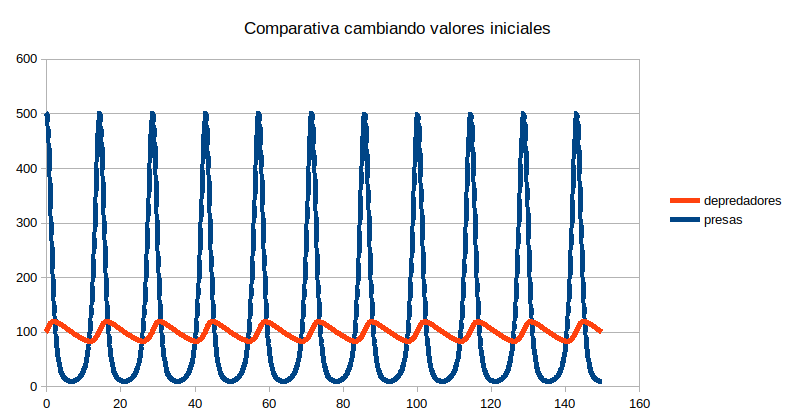
\includegraphics[width=1\linewidth]{images/ejercicio4_4_1}
		\caption{}
	\label{fig:ejercicio441}
	\end{subfigure}%
	\begin{subfigure}{.5\textwidth}
		\centering
	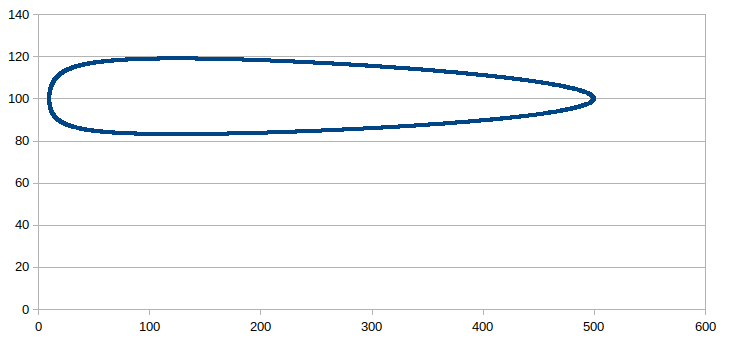
\includegraphics[width=1\linewidth]{images/ejercicio4_4_2}
		\caption{}
	\label{fig:ejercicio442}
	\end{subfigure}
	
	\label{fig:ejercicio44}
\end{figure}
Finalmente al tener una longevidad mayor, podemos ver como la población de depredadores disminuye mucho mas despacio que antes. Al durar mas tiempo, los depredadores tienen que cazar mas y por lo tanto la población de presas también desciende. Aunque a pesar de como hemos visto en experimentos anteriores, este decrecimiento se realiza, aunque de forma brusca, mucho mas suave que en las veces anteriores. Esto se puede deber aunque los depredadores sigan cazando, también siguen muriendo.
\section{Comparación de los distintos metodos de integración}
En todos los experimentos anteriores hemos usado el método Runge-Kutta y ahora compararemos ese metodo con el metodo de Euler. El metodo de Euler, es una forma muy fácil de implementar, tiene el problema de que nos da un error de precisión muy alto. En cambio el metodo usado anteriormente, Runge-Kutta, nos da un error muy bajo pero por contra tiene una dificultad mayor de implementación. \\\newpage
Para hacer el experimento fijaremos los parámetros sin que el modelo sea estable, para poder ver como afecta. Así que la configuración sera la siguiente:
\begin{itemize}
	\item $a_{11} = 5 $
	\item $a_{12} = 0.05$
	\item $a_{21} = 0.0004$
	\item $a_{22} = 0.2$
	\item $x = 500$
	\item $y = 150$ 
\end{itemize}
Y el intervalo de derivación, es decir la \textbf{h} iremos cambiándolo como nos pide en el guión. \\
En la Figura \ref{ejercicio51}  estamos viendo los resultados de usar un $h=0.1$. Usando este intervalo el metodo Runge-Kutta funciona a la perfección ya que nos encontramos lo que a priori pensamos que es lo logico. En cambio en el metodo de Euler, podemos ver que llega un momento en el que el valor de las presas se va al infinito. Esto tiene una simple explicación, y es que llega un momento en el que el error acumulado es tanto que el valor se va al infinito porque se acumulan demasiadas presas. 
\begin{figure}[H]
	\centering
	\begin{subfigure}{.5\textwidth}
		\centering
	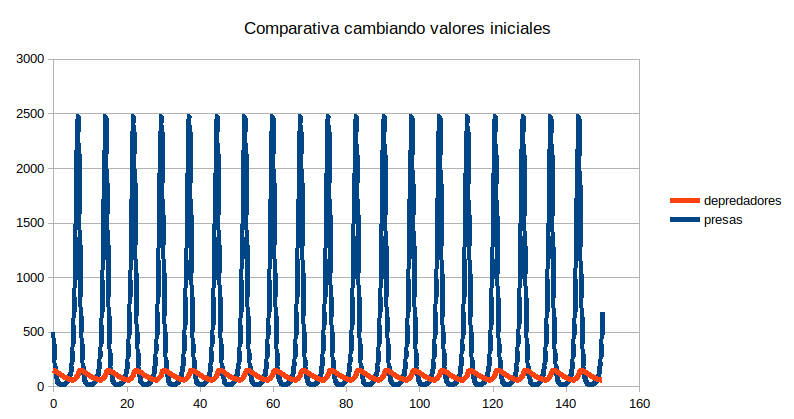
\includegraphics[width=1\linewidth]{images/ejercicio5_5_1}
		\caption{}
	\label{fig:ejercicio551}
	\end{subfigure}%
	\begin{subfigure}{.5\textwidth}
		\centering
	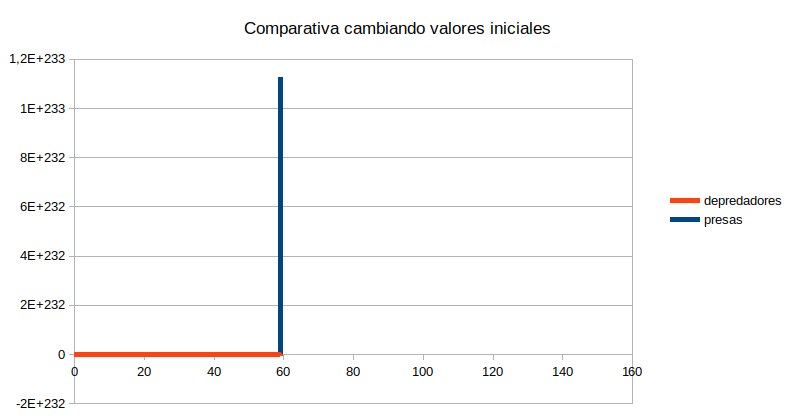
\includegraphics[width=1\linewidth]{images/ejercicio5_1_2}
		\caption{}
	\label{fig:ejercicio512}
	\end{subfigure}
	
	\label{fig:ejercicio51}
\end{figure}

En la Figura \ref{ig:ejercicio53} estamos realizando el experimento con un valor de $h=0.05$. Aunque parece que ya tarda mucho mas en irse el valor de presas al infinito, también podemos ver que periódicamente va fluctuando. Así que todavía no estamos teniendo resultado que se parezcan a los obtenidos en Rugen-Kutta, que si nos da valores que al menos en la grafica parecen bastante adecuados. 
\begin{figure}[H]
	\centering
	\begin{subfigure}{.5\textwidth}
		\centering
	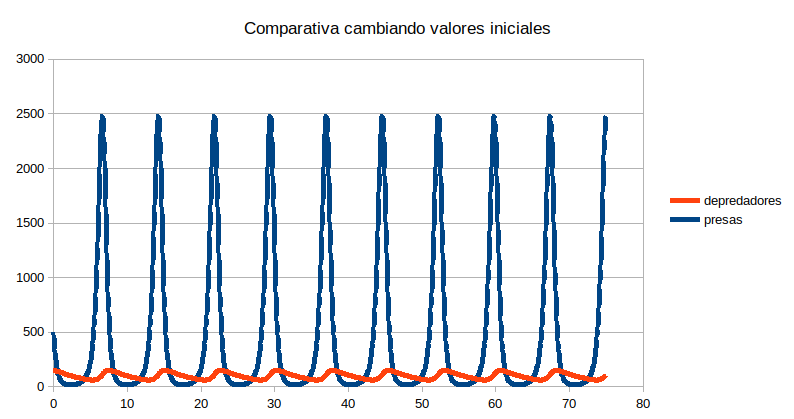
\includegraphics[width=1\linewidth]{images/ejercicio5_3_1}
		\caption{}
	\label{fig:ejercicio531}
	\end{subfigure}%
	\begin{subfigure}{.5\textwidth}
		\centering
	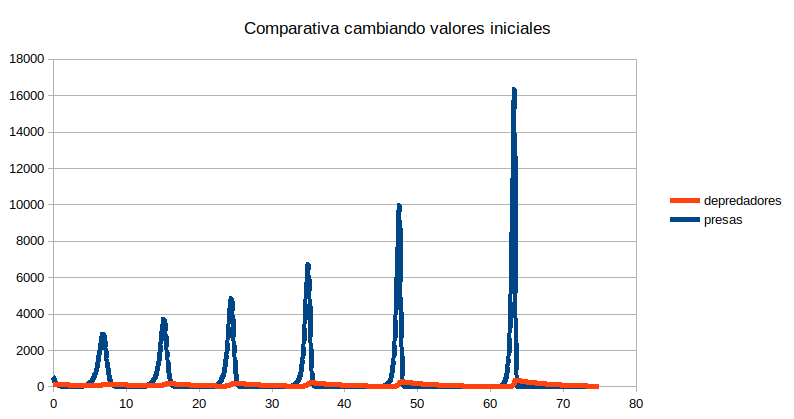
\includegraphics[width=1\linewidth]{images/ejercicio5_3_2}
		\caption{}
	\label{fig:ejercicio532}
	\end{subfigure}
	
	\label{fig:ejercicio53}
\end{figure}
Por ultimo realizamos el experimento usando un valor $h=0.01$, los resultados del experimento los podemos ver en la Figura \ref{fig:ejercicio54}. Aquí los valores de ambas simulaciones son claramente erróneos. Ninguno de los dos nos da resultados a los que esperábamos intuitivamente. No obstante, ambos resultado ahora son muy parecidos, de hecho son casi indistinguibles. 
\begin{figure}[H]
	\centering
	\begin{subfigure}{.5\textwidth}
		\centering
	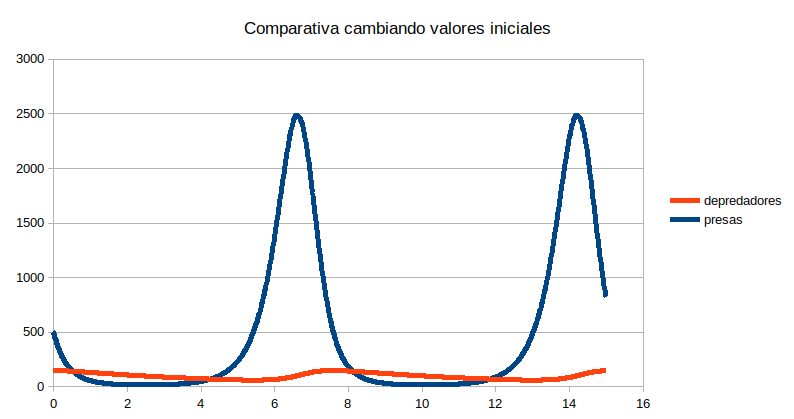
\includegraphics[width=1\linewidth]{images/ejercicio5_4_1}
		\caption{}
	\label{fig:ejercicio541}
	\end{subfigure}%
	\begin{subfigure}{.5\textwidth}
		\centering
	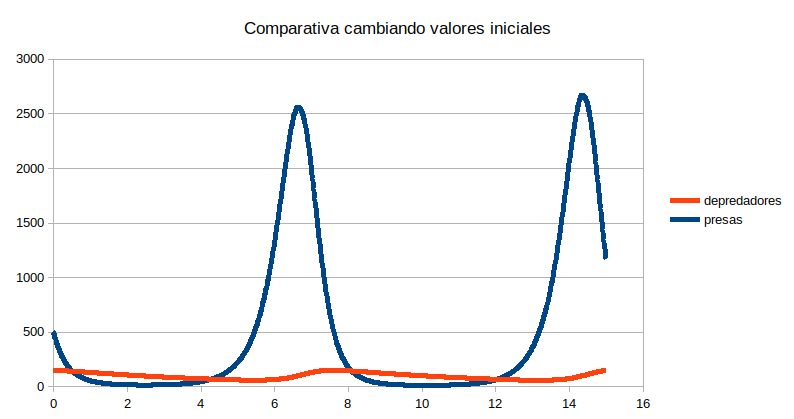
\includegraphics[width=1\linewidth]{images/ejercicio5_4_2}
		\caption{}
	\label{fig:ejercicio542}
	\end{subfigure}
	
	\label{fig:ejercicio54}
\end{figure}

Como conclusión, si tuviera que quedarme con un método seria con Runge-Kutta. Apesar de su complejidad este metodo ofrece muy buenos resultados y con muy poco error. 

\end{document}
	